\documentclass[conference, 11pt]{IEEEtran} 
\usepackage{verbatim}
\usepackage{multirow} \usepackage{enumerate}
\usepackage{amsmath,enumerate} \usepackage{amsthm}
\usepackage{algcompatible}
\usepackage{algpseudocode}
\usepackage{algorithm}
%\usepackage{algorithmic}
\usepackage{pstricks}
\usepackage{amssymb, latexsym}
\usepackage{xfrac}
\usepackage{mathtools}
\usepackage{graphicx}
\usepackage{subfig}
\DeclareGraphicsRule{*}{mps}{*}{}
\usepackage{listings}

%specific to this document only
\usepackage{pgfplots}
\usepackage{pgfplotstable}
\pgfplotstableread{plts/experiment8b1_av.tab}\averageone
\pgfplotstableread{plts/experiment8b2_av.tab}\averagetwo
\pgfplotstableread{plts/experiment8b3_av.tab}\averagethree
\pgfplotstableread{plts/experiment8b4_av.tab}\averagefour
\pgfplotstableread{plts/experiment9a_av.tab}\stepping
\pgfplotstableread{plts/experiment9a1_av.tab}\steppingone
\pgfplotstableread{plts/experiment9a2_av.tab}\steppingtwo
\pgfplotstableread{plts/experiment9a3_av.tab}\steppingthree
\pgfplotstableread{plts/experiment9a4_av.tab}\steppingfour
\pgfplotstableread{plts/experiment9b1_av.tab}\runningone
\pgfplotstableread{plts/experiment9b2_av.tab}\runningtwo
\pgfplotstableread{plts/experiment9b3_av.tab}\runningthree
\pgfplotstableread{plts/experiment9b4_av.tab}\runningfour
\pgfplotstableread{plts/experiment9b_av.tab}\running
\pgfplotstableread{plts/experiment9c_av.tab}\costcomp
\pgfplotstableread{plts/experiment9c1_av.tab}\costcompone
\pgfplotstableread{plts/experiment9c2_av.tab}\costcomptwo
\pgfplotstableread{plts/experiment9c3_av.tab}\costcompthree
\pgfplotstableread{plts/experiment8b1_rn.tab}\runsone
\pgfplotstableread{plts/experiment8b2_rn.tab}\runstwo
\pgfplotstableread{plts/experiment8b3_rn.tab}\runsthree
\pgfplotstableread{plts/experiment8b4_rn.tab}\runsfour
\pgfplotstableset{
  create on use/density/.style={
    create col/expr={\thisrow{nodes}+\thisrow{links}}}
    }
\pgfplotstableset{
  create on use/delta/.style={
    create col/expr={\thisrow{links}*2}}
    }
\pgfplotstableset{
  create on use/nodebylinks/.style={
    create col/expr={(\thisrow{nodes}*\thisrow{links})}}
    }
\pgfplotscreateplotcyclelist{three}{% 
  every mark/.append style={fill=teal}\\% 
  every mark/.append style={fill=green}\\% 
  every mark/.append style={fill=orange}\\% 
}
\pgfplotscreateplotcyclelist{four}{%
  every mark/.append style={fill=teal}\\%
  every mark/.append style={fill=green}\\%
  every mark/.append style={fill=orange}\\%
  every mark/.append style={fill=pink}\\%
}

%%%%%%%%%%%%%

\usepackage{pgf}
\usepackage{tikz}
\usetikzlibrary{decorations.pathmorphing} % LATEX and plain TEX when using Tik Z
\usetikzlibrary{positioning}
\usetikzlibrary{er}
\usetikzlibrary{automata}
\usetikzlibrary{shapes.geometric}
\tikzstyle{vx}=[draw,circle,fill=white,minimum size=2pt, inner sep=1pt, node distance=15mm]
\tikzstyle{ex}=[draw,rectangle,fill=white,minimum size=2pt, inner sep=3pt, node distance=15mm]
\tikzstyle{bup}=[semithick, decoration={bent, aspect=.3, amplitude=4}, decorate, ->, >=stealth]
\tikzstyle{bdn}=[semithick, decoration={bent, aspect=.3, amplitude=-4}, decorate, ->, >=stealth]
\tikzstyle{BUP}=[thick, decoration={bent, aspect=.3, amplitude=8}, decorate, ->, >=stealth]
\tikzstyle{BDN}=[thick, decoration={bent, aspect=.3, amplitude=-8}, decorate, ->, >=stealth]
\tikzstyle{MUP}=[thick, decoration={bent, aspect=.3, amplitude=16}, decorate, ->, >=stealth]
\tikzstyle{MDN}=[thick, decoration={bent, aspect=.3, amplitude=-16}, decorate, ->, >=stealth]
\tikzstyle{str}=[semithick, decorate, ->, >=stealth]
\tikzstyle{cr}=[draw, circle, fill=black!25,minimum size=150pt]

%styles for plots?
\tikzstyle{bls}=[blue, solid, mark=square*]
\tikzstyle{grt}=[red, solid, mark=*]
% \paperheight=11in \paperwidth=8.5in \textheight=9.0in
% \textwidth=6.5in \voffset=-.875in \hoffset=-.875in
\newenvironment{code} {\begin {quote}\begin{footnotesize}}
    {\end{footnotesize}\end{quote}}

% \oddsidemargin 0.0 in \evensidemargin 0.0 in
\newenvironment{enumeratealpha}
{\begin{enumerate}[(a{\textup{)}}]}{\end{enumerate}}

\theoremstyle{plain}
\newtheorem{lem-rule}{Rule}
\newtheorem{thm}{Theorem}
\newtheorem{lem}{Lemma}[thm]
\newtheorem{prop}{Proposition}[thm]
\newtheorem{lprp}{Proposition}[lem]
\theoremstyle{definition}
\newtheorem{defn}{Definition}[thm]
\newtheorem{dfn}{Definitions}[thm]
\newtheorem{ldef}{Definition}
\theoremstyle{remark}
\newtheorem{smy}{Summary}
\newtheorem{note}{Note}[thm]

%algorithms commands
\algblockdefx[Case]{Case}{EndCase} %
[1] [{\em var}] {{\bfseries case} {\em #1\ } } %
{{\bfseries end case}}%
\algcblockdefx[Case]{Case}{When}{EndCase}
[1] [{\em true}] {{\bfseries when} {\em #1\ }}
{{\bfseries end case}} %

\algblockdefx[TimesDo] {DoTimes}{EndTimes}
[1] [0] {#1 times {\bfseries do}}
{{\bfseries end do}}

%subalgorithms environment
\makeatletter
\newcounter{parentalgorithm}
\newenvironment{subalgorithms}{%
%  \refstepcounter{algorithm}%
  \floatname{algorithm}{Procedure}
  \protected@edef\theparentalgorithm{\thealgorithm}%
  \setcounter{parentalgorithm}{\value{algorithm}}%
  \setcounter{algorithm}{0}%
  \def\thealgorithm{\theparentalgorithm-\alph{algorithm}}%
  \ignorespaces
}{%
  \setcounter{algorithm}{\value{parentalgorithm}}%
  \ignorespacesafterend
}
\makeatother

%code environments
\usepackage{float}
 
\floatstyle{ruled}
\newfloat{codeblock}{thp}{lop}
\floatname{codeblock}{Example}

\lstnewenvironment{rubyblock} 
{\lstset{language=Ruby, basicstyle=\small, xleftmargin=10pt, numbers=left, numberstyle=\tiny, stepnumber=2, numbersep=5pt}}
{}
% text macros
\def\cI{{\mathcal I}} \def\cR{{\mathcal R}} \def\cE{{\mathcal E}}
\def\cC{{\mathcal C}} \def\cF{{\mathcal F}} \def\cU{{\mathcal U}}
\def\cH{{\mathcal H}} \def\cD{{\mathcal D}} \def\cB{{\mathcal B}}
\def\cQ{{\mathcal Q}} \def\cV{{\mathcal V}} \def\cS{{\mathcal S}}
\def\cG{{\mathcal G}} \def\cA{{\mathcal A}} \def\cO{{\mathcal O}}
\def\cW{{\mathcal W}} \def\cL{{\mathcal L}} 

\def\bI{{\mathbb I}} \def\bO{{\mathbb O}}
\def\bC{{\mathbb C}} \def\bM{{\mathbb M}}
\def\bId{{$\mathbb I$}} \def\bOd{{$\mathbb O$}}
\def\bCd{{$\mathbb C$}} \def\bMd{{$\mathbb M$}}

\def\cId{{$\mathcal I$}} \def\cRd{{$\mathcal R$}} \def\cEd{{$\mathcal E$}} 
\def\cCd{{$\mathcal C$}} \def\cFd{{$\mathcal F$}} \def\cUd{{$\mathcal U$}} 
\def\cHd{{$\mathcal H$}} \def\cDd{{$\mathcal D$}} \def\cBd{{$\mathcal B$}} 
\def\cQd{{$\mathcal Q$}} \def\cVd{{$\mathcal V$}} \def\cSd{{$\mathcal S$}} 
\def\cGd{{$\mathcal G$}} \def\cAd{{$\mathcal A$}} \def\cOd{{$\mathcal O$}}
\def\cWd{{$\mathcal W$}} \def\cLd{{$\mathcal L$}}

\bibliographystyle {IEEEtranS}

\begin{document}
\title{Distributed Vertex Cover in Graphs} 

\author{\IEEEauthorblockN{J. Paul Daigle, Sushil K. Prasad}
\IEEEauthorblockA{Department of Computer Science\\
Georgia State University\\
Atlanta, Georgia 30303\\
Email: jdaigle1@student.gsu.edu, sprasad@gsu.edu}
}

\maketitle

\begin{abstract}
 Vertex cover, a minimal set of nodes to cover all edges in a graph, is an abstraction of coverage problems in sensor networks, transportation networks, etc, and is a well-konwn NP-hard problem.  Minimum weighted vertex cover (MWVC) problem asks for further minimizing the cumulative weight of a vertex cover.  We present new distributed k-hop algorithms for MWVC problem with theoretical and practical values.  Our first 1-hop approximation algorithm, based on matching a maximal set of non-adjacent edges, is provably 2-optimal with a communication complexity of $\log n$.   It compares very well with the current state-of-art in quality while significantly reducing communication cost.

We also explore an important variant, the problem of finding a series of vertex covers to maximize network lifetime.  Our second algorithm, based on a key insight into the vertex cover problem of collecting partial covers from 2-hop neighbors, is an excellent practical algorithm.  It is representative of a problem-structure based efficient sampling algorithm in the exponential size local solution space.   We show that a partial cover based algorithm can be enhanced further to compete very well and exceed the lifetime obtained with state-of-the-art algorithms. 
\end{abstract}
\section{Introduction}
The Minimum Vertex Cover problem and its weighted variant are NP-Complete problems with several known linear time sequential algorithms that provide constant approximations. The existence of such algorithms suggests that there is a constant time distributed algorithm that would provide a constant approximation for MVC or MWVC, but it has been shown that a constant approximation of MWVC cannot be found by a distributed algorithm in a constant number of rounds.\cite{1011811} 

Here we present a distributed two-approximate algorithm to solve MWVC in an expected running time of $O(logn)$, based on the linear time sequential algorithm of Gonzalez.\cite{Gonzalez1995129} This is not the first such algorithm to appear in the literature, but there are implementation advantages to our approach. In addition, we present an interesting subroutine that runs in constant time and improves the quality of solutions for both our algorithm and the prior algorithm of Koufogiannakis and Young.\cite{1582746} This subroutine turns out to have practical value when applied to the related problem of sensor network lifetime. 

All of the distributed algorithms described are assumed to be running on a message passing model, the compute nodes are mapped to the vertexes of the graph, and the edges of the graph represent viable paths for communication between nodes. 

\section{Prior Work}

Linear time algorithms for covering problems are surveyed in detail in \cite{254190}. Linear Programming techniques for constant ratio approximation of MWVC were developed by Bar-Yehuda and Even in 1981 \cite{Bar-Yehuda:1981lr,:fk}. Gonzalez created an LP-Free linear time algorithm based on Maximal Matching in 1995 which is the basis of our distributed algorithm \cite{Gonzalez1995129}. 

Maximal Matching also forms the basis for the 2-approximate distributed MWVC algorithm developed by Grandoni et. al \cite{1435381}. A simpler algorithm was presented by Koufaganis and Young in 2009 \cite{1582746}. 

\section{Definitions}
The coverage problems in this paper are common coverage problems which are known to be NP-Complete. For convenience, the problem definitions are provided here.

\subsubsection{Minimum Vertex Cover (MVC)}
\label{sub:mvc}
Given an undirected Graph $G(V,E)$, a {\em Vertex Cover} of $G$ is a set of vertices $V'$ such that for each edge $e_{u,v} \in E$, $u \in V'$ or $v \in V'$. The Minimum Vertex Cover Problem is to find the smallest possible vertex cover of $G$.

\subsubsection{Minimum Weighted Vertex Cover (MWVC)}
\label{sub:mwvc}
Given an undirected Graph $G(V,E)$, where each $v \in V$ has a positive weight $w(v)$, minimize $\sum_{v \in V'} w(v)$.

%\subsubsection{Minimum (Weighted) Vertex Cover of a Hypergraph}

%Given a Hypergraph $G(V,E)$, with vertices $v \in V$ and hyperedges $e_{v_1...v_n}$, a vertex cover of $G$ is a set $V'\: | \: \forall e \in E,\quad \exists v \in V'\: |\: v \in e$. The minimum vertex cover and minimum weighted vertex cover are as described in sections~\ref{sub:mvc} and ~\ref{sub:mwvc}


\section{Algorithms}
\label{sec:algorithms}

\subsection{Distributed Generalized Maximal Matching Algorithm}
\subsubsection{Description}
Algorithm~\ref{alg:dgmm} is our distributed implementation of the 2-approximate minimum weighted vertex cover algorithm presented by Gonzalez.\cite{Gonzalez1995129} The Gonzalez algorithm proceeds by selecting each edge in turn and choosing one of the endpoints of that edge to add to the cover. The sequential algorithm goes through each edge in turn and assigns the edge a weight according to equation~\ref{eqn:gmm}. If the weight of a vertex is equal to the sum of it's incident edge weights, that vertex is added to the cover. 

\begin{equation}
  \label{eqn:gmm}
  w(e(u,v)) = min 
  \begin{dcases} 
    w(u) - \sum_{i \ne v} w(e(u,i)) \\
    w(v) - \sum_{i \ne u} w(e(i,v)) 
  \end{dcases}    
\end{equation}

The distributed version of the algorithm chooses some disjoint set of edges and assigns weights as described. The precise method of choosing edges and updating weights is given in Algorithm~\ref{alg:dgmm}. The general progress of the algorithm is defined by the automata in Figure~\ref{fig:dgmm-auto}. Each vertex begins in the \cCd state, and chooses to either send invitations (\cId), or listen for invitation (\cLd). Vertexes in the \cId state choose one neighbor to send an invitation to and transition to a waiting state (\cWd), and vertexes in the \cLd state choose one invitation to accept. The acceptence message is sent during the response state \cRd. All vertexes then update their status (\cUd). Vertexes that have either chosen to join the cover or which have no undecided neighbors will transition to the done state, (\cDd), and other vertexes return to state \cCd.  

\begin{figure}[htp]
  \caption{DGMM Automata}
  \begin{center}
  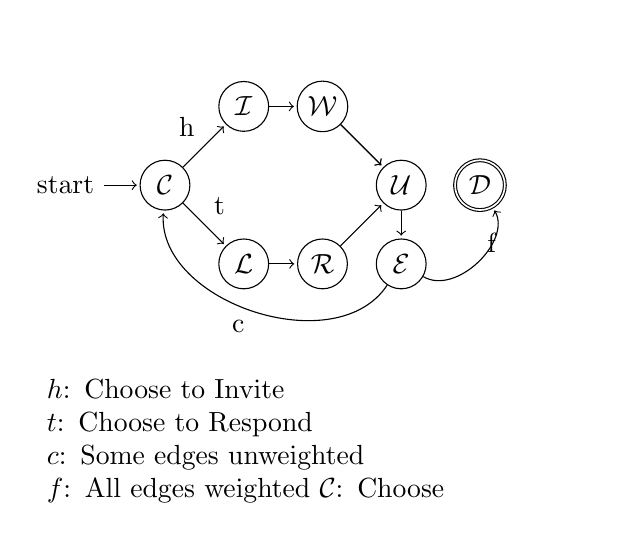
\begin{tikzpicture}[shorten >=1pt,node distance=1cm,on grid,auto, bend angle=75, every state/.style={scale=1, minimum size=18pt, inner sep=2pt}]
    %\draw [help lines] (0,-2) grid (4,2);
    \path [help lines] (0,-2) grid (4,2); 
    \node [state, initial]   (C)          {\cCd};
    \node [state] (I)            at (1,1) {\cId};
    \node [state] (L)            at (1,-1) {\cLd};
    \node [state] (W)            at (2,1)       {\cWd};
    \node [state] (R)            at (2,-1)       {\cRd};
    \node [state] (U)            at (3,0) {\cUd};
    \node [state] (E)            at (3,-1)       {\cEd};
    \node [state, accepting] (D) at (4,0)   {\cDd};

    \path [->] (C) edge              node {h} (I)
                   edge              node {t} (L)
               (L) edge              node {} (R)
               (I) edge              node {} (W)
               (W) edge              node {} (U)
               (R) edge              node {} (U)
               (U) edge              node {} (E);
    \path [->] (E) edge [bend right] node [above right] {f} (D);
    \path [->] (W) edge              node {} (U);
    \path [->] (E) edge [bend left]  node {c} (C);


      \node [text width=7cm] (key) at (2, -3.25) {
	$h$: Choose to Invite \hspace{4cm}
        $t$: Choose to Respond\hspace{4cm}
        $c$: Some edges unweighted\hspace{5cm}
	$f$: All edges weighted
	$\cC$: Choose 
	}; 
  \end{tikzpicture}
  \end{center}
  \label{fig:dgmm-auto}
\end{figure}


During the \cUd state, vertex pairs formed during the invitation/acceptance phases are able to assign a weight to the edge between them independently using equation~\ref{eqn:gmm}, and therefore decide whether or not to join the cover. During the \cEd stage neighboring vertexes are able to update some of their own edge weights, by assigning a weight of zero to any edges incident to a vertex which has joined the cover.

\begin{algorithm}
\caption{Distributed Weighted Vertex Cover}
\begin{algorithmic}
\Require {$G(V,E)$: a graph}
\ForAll {$v_u \in V$ in parrallel}
\State $S_u \leftarrow False$
\State state $\leftarrow$ Choose
\Repeat
\State Broadcast $S_u$
\If {$S_v = True$ for $v_v$ incident to self}
\State Set Weight $e_{u,v} \leftarrow 0$
\EndIf
\If {state = Choose}
\State {Choose A State (Invite, Listen)}
\ElsIf {state = Invite}
\State {Select an unweighted edge, $e_{u,v}$}
\State {Broadcast an Invitation to $v_v$}
\State {state $\leftarrow$ Wait}
\ElsIf {state = Listen}
\State {Collect Invitations}
\State {state $\leftarrow$ Respond}
\ElsIf {state = Wait}
\State {Collect Responses}
\If {Response Matches Invitation}
\State {Update Weight $e_{u,v}$}
\If {$\sum_{w_e} e incident v_u = w_u$}
\State $S_u \leftarrow true$
\EndIf
\EndIf
\State {state $\leftarrow$ Choose}
\ElsIf {state = Respond}
\State Choose Invitation, Broadcast Response
\State {Update Weight $e_{u,v}$}
\If {$\sum_{w_e} e incident v_u = w_u$}
\State $S_u \leftarrow true$
\EndIf
\State {state $\leftarrow$ Choose}
\EndIf
\Until {$S_u = true$ OR $S_v = true$ for all $v_v$ incident $v_u$}
\EndFor
\end{algorithmic}
\label{alg:dgmm}
\end{algorithm}

\subsubsection{Proof of 2-Approximation}
The sequential version of Algorithm~\ref{alg:dgmm} has been shown to be 2-approximate for any ordering of edges. The distributed version can never select contiguous edges in a single round, as each node can form at most one partnership in a round. Because The simultaneous selection of vertexes to join the cover based on disjoint edges is exactly equivalent to the sequential selection of vertexes by selecting each edge under consideration in turn.\footnote{This algorithm could therefore also be used to provide an edge coloring in approximately the same time, equivalent to a greedy linear algorithm.}


\subsection{Redundancy Checking}

When vertexes make local decisions to join a cover, it is difficult to judge whether any neighbor will also decide to join the cover. In some cases, this leads to vertexes joining the cover which can be subsequently removed while still retaining full coverage. Removing these nodes will certainly reduce the total weight of the cover. We therefore implement a {\em redundancy checking} algorithm for Vertex Cover. Figure~\ref{fig:red} shows the progression of Algorithm~\ref{alg:red}.

\begin{figure}[htp]
  \begin{center}
    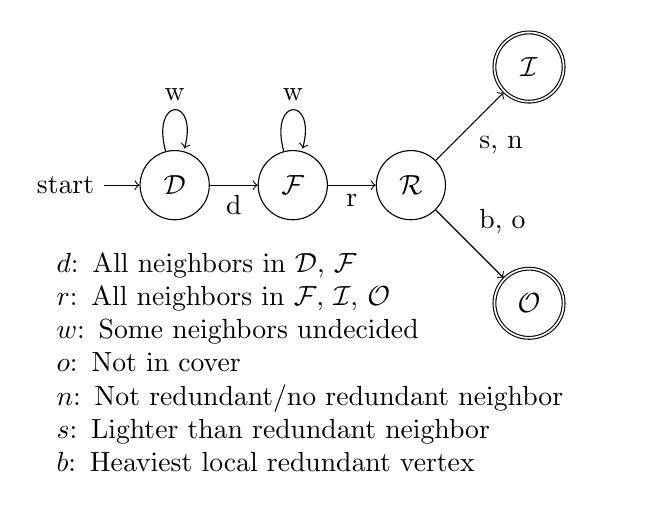
\begin{tikzpicture}
     % \draw[help lines] (0, -2) grid (5,2);
      \path [help lines] (0, -2) grid (5,2);
      \node [state, initial] (D) {\cDd};
      \node [state] (F) at (1.5, 0) {\cFd};
      \node [state] (R) at (3, 0) {\cRd};
      \node [state, accepting] (I) at (4.5, 1.5) {\cId};
      \node [state, accepting] (O) at (4.5, -1.5) {\cOd};

      \path [->] (D) edge node [below] {d} (F)
                     edge [loop above] node {w} ()
                 (F) edge node [below] {r} (R)
                     edge [loop above] node {w} ()
                 (R) edge node [above right]{b, o} (O)
                     edge node [below right]{s, n} (I);
      \node [text width=7cm] (key) at (2, -2.25) {$d$: All neighbors in \cDd, \cFd \hspace{4cm}
        $r$: All neighbors in \cFd, \cId, \cOd  \hspace{4cm}
        $w$: Some neighbors undecided  \hspace{5cm}
        $o$: Not in cover \hspace{5cm}
        $n$: Not redundant/no redundant neighbor  \hspace{4cm}
        $s$: Lighter than redundant neighbor  \hspace{4cm}
        $b$: Heaviest local redundant vertex  \hspace{4cm}};
                     
    \end{tikzpicture}
    \caption{Redundancy Checking Algorithm}
    \label{fig:red}
  \end{center}
\end{figure} 

\begin{algorithm}
\caption{ Redundancy checking algorithm (RC)} 
\begin{algorithmic}[1]
  \Require {$G(V,E), w(v)$: A vertex-weighted graph}
  \Require {state$(v_v) =  \cD \vee \cF$} \Comment See Fig~\ref{fig:red}
  \Ensure {state$(v_v) = (\cI \vee \cO)$}
  \ForAll {$v_v \in V$ synchronously}
  \If {state $=$ \cDd}
  \State {DO check-finished}
  \ElsIf {state $=$ \cFd}
  \State {DO check-redundant}
  \EndIf
  \EndFor
  \Procedure{check-finished}{}
  \If {$\forall v_u$ incident $v_v$, state$(v_u) = \cD \vee \cF$}
  \If {$v_v \in \bC$} \Comment Where \bCd\ is the Cover
  \If {$\forall v_u$ incident $v_v, v_n \in \bC$}
  \State {redundant $\gets$ TRUE}
  \EndIf
  \State {state $\gets$ \cFd}
  \EndIf
  \Else 
  \State {state $\gets$ \cDd}
  \EndIf
  \EndProcedure
  \Procedure{check-redundant}{}
  \If {$\forall v_u$ incident $v_v$, state$(v_u) = \cF \vee \cI \vee \cO)$}
  \If {redundant $=$ TRUE}
  \If {$\forall v_u$ incident $v_v$, redundant$(v_u) =$ FALSE}
  \State {remove $v_v$ from \bCd}
  \Else
  \State {$a \gets [w(v_v)] + [w(v_u) \forall v_u$ incident $v_v]$}
  \If {maximum of $a = v_v$} \Comment {$v_v$ has the largest weight in its neighborhood}
  \State {remove $v_v$ from \bCd}
  \EndIf
  \EndIf
  \EndIf
  \State {state $\gets \cI \vee \cO$}
  \Else
  \State {state $\gets$ \cFd}
  \EndIf
  \EndProcedure
\end{algorithmic}
\label{alg:red}
\end{algorithm}


The concept behind Algorithm~\ref{alg:red} is simple, a vertex that does not have any edges covered by a vertex of greater weight removes itself from the cover. This simple idea provides some results in another context. When examining target coverage in a sensor network, most current algorithms ignore the communication cost of establishing the target cover\cite{1514028}. One reason for this is that the cost is generally considered to be a constant, that is, any algorithm that provides continuous coverage must perform a global reshuffle periodically in order to maximize network lifetime. 

Redundancy removal provides a tool to circumvent this problem. As each sensor reaches the end of its battery life, it can tell its neighbors to turn on. These neighbors can then negotiate with their neighbors, with redundant sensors turning off. The advantage of this approach is two-fold. First, there are no global reshuffle rounds. Communication costs are only incurred when strictly necessary to maintain the network. Second, sensors which are not affected by a particular event--those that are three or more hops away from a dying sensor--do not incur any extra cost as a result of a specific event.

Depending on the deployment details of a given network, communication costs may be much higher than sensing costs, so using redundancy checking as a means of network maintenance may extend network lifetimes. In section~\ref{sec:experiment}, we explore this potential through simulation.


\subsection{Partial Cover Dependency Graph}
\label{sec:life-depend}
Target Coverage and Minimum Weighted Vertex Cover are both NP-Complete problems. It has also been proved that MWVC cannot be approximated to a constant factor locally within any constant number of communication rounds~\cite{1011811}, and as we have shown this limitation must apply to target coverage as well. The Dependency Graph is a heuristic framework for such problems~\cite{IPDPS.2008.45361}. It has been shown to produce good results when applied to the Lifetime Maximization problem in sensor networks~\cite{978-3-540-89894-8_26}.

The framework applies to problems where local solutions can be combined to form a feasible global solution. The essential steps of the framework are: 
\begin{enumerate}
\item Establish that combined local solutions lead to a feasible global solution
\item Model the state space of the local solutions
\item Determine a priority heuristic for local solutions
\item Design a reasonable negotiating strategy between neighbors
\end{enumerate} 
A detailed description of each of these steps can be found in~\cite{IPDPS.2008.45361}.

The application of the framework relies on dependencies between local solutions. In the case of the MWVC problem, there are several approaches that can be taken to determine what a local solution is. The simplest approach is to have each vertex only consider edges incident to itself. Naively, each vertex would have exactly two local solutions, the cover containing itself and the cover containing all of its neighbors. However, it is trivial to construct graphs, such as the 4-clique, in which no solution would be possible with these constraints. So even for this simple case, a large number of possible covers have to be considered. The number of possible local covers for a vertex of degree $\Delta$ is $\sum_{i=0}^\Delta \binom{\Delta}{i}$.

\subsubsection{Dependency Graph}
Given a Weighted Graph $G(V,E)$, a {\em Dependency Graph} $H(S,D)$ for $v \in V$ is defined by local solutions $s \in S$ and dependencies $d_{u,v} \in D$ between those solutions. In the case of the MWVC, each solution is made up of a set of vertices that cover the edges incident to $v$. The goal is to use the local solutions to build $\cC$, a vertex cover of $G$. The initial dependency graph for each vertex $v$ consists of the set containing the vertex $\{v\}$, and the set containing the neighbors of $v$, $\{n_v)\}$. 

\subsection{Prioritizing Local Solutions}

Given two local covers $c_1, c_2$, we define the degree of a cover ($w(c)$) as $\sum w(v)\:|\: v \in c, v \notin \cC$.  

\subsection{Negotiation Strategies}
Initially, each vertex $v$ is only aware of two solutions, the solution containing itself $s_s$ and the solution containing all of its neighbors $s_n$, which have no dependencies between them. In order to ensure 2-approximation, $v$ can only safely join $\cC$ if its own weight $w_v$ is at most half of the cumulative weight of all $w_u, u \in s_n $. If that condition cannot be met, then a vertex can join $\cC$ if it is the smallest node in it's local neighborhood not in $\cC$. A vertex that cannot meet either of these conditions waits for the next round. 

Some nodes will turn on, and in doing so will create new covers for their neighbors. At the beginning of each round, each vertex notes whether any vertexes in $s_n$ have joined $\cC$, and if so, it creates a new solution $s$ composed of itself and those vertexes. This solution will have a dependency to both $s_s$ and $s_n$, and the decision criteria can be applied to this new solution. 

\subsection{Partial Cover Dependency Graph}

The number of local covers increases as a function of the density of the local neighborhood. If $\Delta$ is small, this is not a problem, but as $\Delta$ increases the number of potential local covers increases rapidly. The Partial Cover Dependency Graph samples this exponential space and reduces the number of solutions to $\Delta$. A given vertex can only see two covers for it's own edges: the cover containing itself, and the cover containing all of its neighbors. The partial cover dependency graph samples the solution space based on what vertexes would have to be on if either of these two covers were off. 

\subsubsection{Construction of the PCDG}

Given a graph $G(V,E)$, for each vertex in $V$ we can define a partial cover dependency graph consisting of the {\em partial cover pair} $\cC_v, \cC_{n(v)}$ for v, and the partial cover pair for each neighbor of v. Given a node $v \in V$, $\cC_v$ consists of v and its two-hop neighbors, while $\cC_{n(v)}$ consists of $v$'s one-hop neighbors. For clarity, we define terms below.

\begin{defn}
One-hop Neighbor of $v$ : $u \in V \mid \exists e(u,v) \in E$
\end{defn}

\begin{defn}
Two-hop Neighbor of $v$ : $u \in V \mid \exists e(u,w) \in E \land \exists e(w,v) \in E \land \neg\exists e(u,v) \in E$
\end{defn}

\begin{defn}
$N_v$ : The set of one-hop neighbors of $v$
\end{defn}
\begin{defn}
$N_v^2$ : The set of two-hop neighbors of $v$
\end{defn}

\begin{defn}
$\cC_v$ : $\{v\} \cup N_v^2$
\end{defn}

\begin{defn}
$\cC_{n(v)}$ : $N_v$
\end{defn} 

\begin{defn}
Partial Cover Dependency Graph of $v$ : a graph $H(C,F)$ such that \begin{align*}& 1. C = \{\cC_v, \cC_{n(v)}\} \cup \{\cC_u, \cC_{n(u)}\} \forall u \in N_v\\ & 2. \exists f(c_1, c_2) \in F \iff \exists u \in V \mid u \in c_1 \land u \in c_2\end{align*}.
\end{defn} 

After constructing $H$, each cover is assigned a {\em weight} and a {\em degree}. The weight of a cover is defined as the sum of the weight of the vertexes in that cover, and the degree is defined by the number of edges for that cover. Figure~\ref{fig:pcdg} shows a graph and the corresponding partial cover dependency graph of a vertex in that graph.

\begin{figure}[htp]
  \begin{center}
  \subfloat[Weighted Graph $G$]
  {  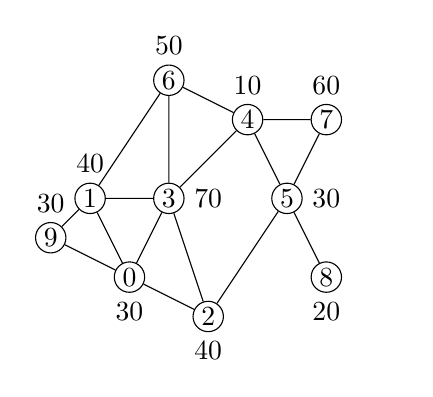
\begin{tikzpicture}
%      \draw [help lines] (0,-2) grid (4,2);
      \path [help lines] (0,-2) grid (4,2); 
      \node [vx, label=below:30]  (0) at (.5,-1) {0};
      \node [vx, label=above:40] (1) at (0, 0) {1};
      \node [vx, label=below:40] (2) at (1.5,-1.5) {2};
      \node [vx, label=right:70] (3) at (1, 0) {3};
      \node [vx, label=above:10] (4) at (2, 1) {4};
      \node [vx, label=right:30] (5) at (2.5, 0) {5};
      \node [vx, label=above:50] (6) at (1, 1.5) {6};
      \node [vx, label=above:60] (7) at (3, 1) {7};
      \node [vx, label=below:20] (8) at (3,-1) {8};
      \node [vx, label=above:30] (9) at (-.5,-.5) {9};
      \path [draw] 
      (0) -- (1)
      (0) -- (2)
      (0) -- (3)
			(0) -- (9)
      (1) -- (3)
      (1) -- (6)
			(1) -- (9)
      (2) -- (3)
      (2) -- (5)
      (3) -- (4)
      (3) -- (6)
      (4) -- (5)
      (4) -- (6)
      (4) -- (7)
      (5) -- (7)
      (5) -- (8);
    \end{tikzpicture}
}
  \\
  \subfloat[PCDG for Vertex 7]{
    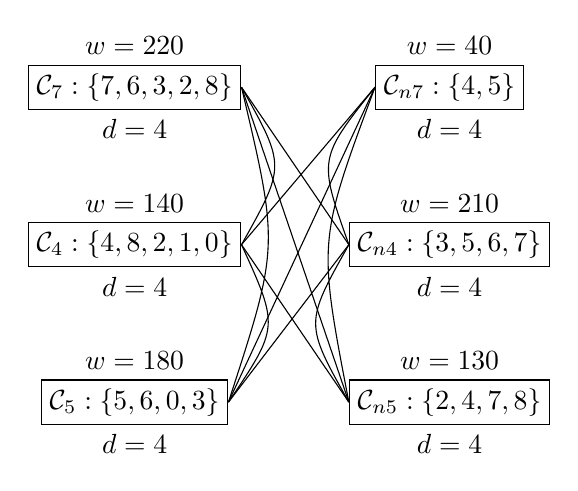
\begin{tikzpicture}
%      \draw [help lines] (0,-3) grid (6,3);
     \path [help lines] (0,-2) grid (4,2);
      \node [ex, label={above: $w=220$}, label={below: $d=4$}] (C7) at (1,2) {$\cC_7: \{7,6,3,2,8\}$};
      \node [ex, label={above: $w=40$}, label={below: $d=4$}] (CN7) at (5,2) {$\cC_{n7}: \{4,5\}$};
      \node [ex, label={above: $w=140$}, label={below: $d=4$}] (C4) at (1,0) {$\cC_4: \{4,8,2,1,0\}$};
      \node [ex, label={above: $w=210$}, label={below: $d=4$}] (CN4) at (5,0) {$\cC_{n4}: \{3,5,6,7\}$};
      \node [ex, label={above: $w=180$}, label={below: $d=4$}] (C5) at (1,-2) {$\cC_5: \{5,6,0,3\}$};
      \node [ex, label={above: $w=130$}, label={below: $d=4$}] (CN5) at (5,-2) {$\cC_{n5}: \{2,4,7,8\}$};

      \path [draw] 
      (C7.east) -- (CN5.west)
      (C7.east) -- (CN4.west)
      (CN4.west) -- (C5.east);
      \path [draw, decoration={bent, amplitude=16}, decorate]
      (C7.east) -- (C5.east)
      (C7.east) -- (C4.east)
      (C4.east) -- (C5.east);
      \path [draw]
      (CN7.west) -- (C5.east)
      (CN7.west) -- (C4.east)
      (CN5.west) -- (C4.east);
      \path [draw, decoration={bent, amplitude=-16}, decorate]
      (CN7.west) -- (CN5.west)
      (CN7.west) -- (CN4.west)
      (CN4.west) -- (CN5.west);
    \end{tikzpicture}
  }
  \end{center}
  \caption{Partial Cover Dependency Graph}
  \label{fig:pcdg}
\end{figure}


\subsubsection{PCDG Algorithm}

The PCDG algorithm uses 3-hop information for immediate setup of the graph, as described in the previous section. After initial setup, the algorithm no longer updates any information beyond 1-hop. Figure~\ref{fig:pcdg_auto} shows the progression of PCDG.
\begin{figure}[htp]
  \begin{center}
    \caption{Partial Cover Dependency Algorithm}
    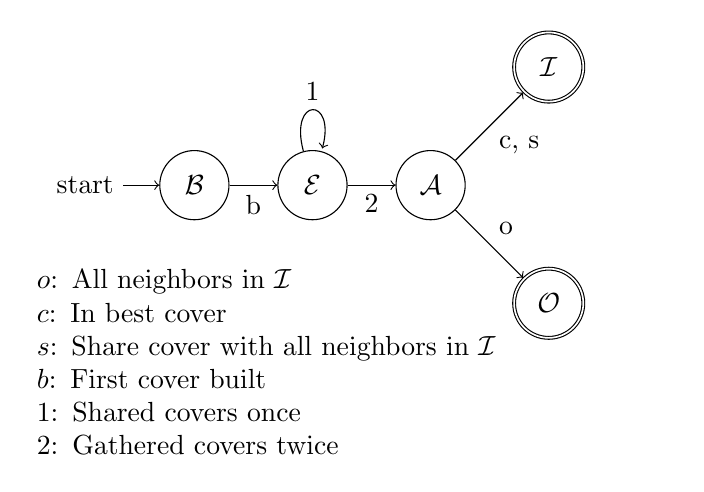
\begin{tikzpicture}
     % \draw[help lines] (0, -2) grid (5,2);
      \path [help lines] (0, -2) grid (5,2);
      \node [state, initial] (B) {\cBd};
      \node [state] (E) at (1.5, 0) {\cEd};
      \node [state] (A) at (3, 0) {\cAd};
      \node [state, accepting] (I) at (4.5, 1.5) {\cId};
      \node [state, accepting] (O) at (4.5, -1.5) {\cOd};

      \path [->] (B) edge node [below] {b} (E)
                 (E) edge node [below] {2} (A)
                     edge [loop above] node {1} ()
                 (A) edge node [above right]{o} (O)
                     edge node [below right]{c, s} (I);
      \node [text width=8cm] (key) at (2, -2.25) {
        $o$: All neighbors in \cId  \hspace{7cm}
        $c$: In best cover  \hspace{7cm}
        $s$: Share cover with all neighbors in \cId \hspace{5cm}
        $b$: First cover built  \hspace{7cm}
        $1$: Shared covers once  \hspace{7cm}
        $2$: Gathered covers twice  \hspace{4cm}};
                     
    \end{tikzpicture}
  \label{fig:red}
  \end{center}
\end{figure}

A key issue in developing algorithms in the Dependency Graph framework is the ranking of covers and the establishment of degrees. We chose a relatively simple method of ranking covers which has given good results. Most interesting, however, is that the initial ranking of covers seems to be superior to all subsequent rankings. This was determined during the experiment phase of our research, which is detailed in the next section.

\section{Experiments}
\label{sec:experiment}
Experiments were conducted to test algorithm performance and examine the relationship between maximizing network lifetime and minimizing vertex cover.
\subsection{Minimum Weighted Vertex Cover}
\label{sub:mwvc-exp}

For the MWVC problem, we tested the DGMM algorithm against a similar algorithm developed in \cite{1582746}. The Koufogiannakis/Young algorithm uses a similar coin flipping mechanism between vertexes, with each one choosing to be a 'root' or a 'leaf' node, and the algorithm proceeds in a way that guarantees that two adjacent nodes making independent decisions will reach the same conclusions. 

\subsection{Target Coverage}

We chose the DEEPS algorithm developed in \cite{1640702} as a benchmark for PCDG. This is a state-of-the art two-hop algorithm which has been demonstrated through simulation and real-world experiments to improve network lifetimes. DEEPS insures network coverage by assigning targets to nodes, preferring the strongest member of weakest sets to take charge. 

DEEPS requires global reshuffles to maintain coverage, and those shuffles are proactive, they take place on a schedule rather than on an as needed basis.

\subsection{Experimental Design}
\label{sub:exp-design}
Random connected graphs were constructed, with the number of nodes and edges as the inputs. Nodes recieved a random weight between 400 and 1000. Graph construction proceeded by a modification of Erlang's method: all possible edges were generated and then random edges were chosen until the desired number of edges had been added to the graph. In order to ensure connectivity, Minimum Spanning Trees were constructed for each graph and connected together until each graph had a single MST. 

The simulator was developed in Ruby. Ruby was chosen primarily because of its strong system of multiple inheritance and the relative ease of unit testing and debugging. The source code for each algorithm and the simulation framework are open source and available for download.\footnote{Using the mercurial VCS, command hg clone https://rvertex.graphcomplexity.googlecode.com/hg/ graphcomplexity-rvertex will retrieve a copy of the code repository. This paper uses revision 67446e3ca7 of the code base} 

For the MWVC problem, graphs were constructed with 120, 240, 480, and 960 vertices with link densities of 1.5, 3, 6, 12, 24, and 48. 50 graphs were generated at each size, and the K/F, DGMM, and the redundant versions of each were run on each generated graph.

For the Target Coverage problem, the difficulty was to capture the communication cost associated with running the covering algorithms. We assume that in every case, a constant amount of energy is required to maintain the sensing and information sharing functions of the network. In our simulation, this cost is only applied to sensors that are on in a given round. The cost of organizing the sensors is a global cost, as every sensor in the network is required to participate in establishing a cover. This is applied as a constant drain on all sensors in the network. We simulate this drain as being on a spectrum from free to being equal to the cost of the information sharing and sensing function of the network. 

We tested PCDG and DEEPS in two scenarios: one where each algorithm performs a global reshuffle in each round, and one where each algorithm sets up an initial cover, and then uses redundancy checking to perform local maintenance on an as needed basis. Graphs were constructed with 20, 40, and 80 vertices and link densities of 1.5, 3, and 6. 25 experiments were run for each graph size.
 
\subsection{Experimental Results}
\label{sub:exp-results}
\subsubsection{Minimum Weighted Vertex Cover}
\label{sub:mwvc-results}
As expected, the addition of the constant time redundancy check improved results for both the DGMM algorithm and the K/F algorithm. Figures~\ref{plt:match} and~\ref{plt:star} show the improvement. In our experiments the affect was small on average, less than 10\%, but this could be viewed as significant given the low cost of the routine. 
\begin{figure}[htp]
\begin{center}
\begin{tikzpicture}
  \begin{axis}[xlabel=Average Degree, ylabel=Total Weight, legend style={at={(1,0.25)}, anchor=east}, cycle list name={four} ]
    \addplot+[bls] table [x=links, y=mat-reg]{\averageone};
    \addplot+[bls] table [x=links, y=mat-reg]{\averagetwo};
    \addplot+[bls] table [x=links, y=mat-reg]{\averagethree};
    \addplot+[bls] table [x=links, y=mat-reg]{\averagefour};
    \addplot+[grt] table [x=links, y=mat-red]{\averageone};
    \addplot+[grt] table [x=links, y=mat-red]{\averagetwo};
    \addplot+[grt] table [x=links, y=mat-red]{\averagethree};
    \addplot+[grt] table [x=links, y=mat-red]{\averagefour};
    \legend{Match,,,, Match+R}
  \end{axis}
\end{tikzpicture}
\caption{Redundancy Applied to Matching}
\label{plt:match}
\end{center}
\end{figure}
\begin{figure}[htp]
\begin{center}
\begin{tikzpicture}
  \begin{axis}[xlabel=Average Degree, ylabel=Total Weight, legend style={at={(.95,0.75)}, anchor=north east}, cycle list name={four}]
    \addplot+[bls] table [x=links, y=star-reg]{\averageone};
    \addplot+[bls] table [x=links, y=star-reg]{\averagetwo};
    \addplot+[bls] table [x=links, y=star-reg]{\averagethree};
    \addplot+[bls] table [x=links, y=star-reg]{\averagefour};
    \addplot+[grt] table [x=links, y=star-red]{\averageone};
    \addplot+[grt] table [x=links, y=star-red]{\averagetwo};
    \addplot+[grt] table [x=links, y=star-red]{\averagethree};
    \addplot+[grt] table [x=links, y=star-red]{\averagefour};
    \legend{K/Y,,,, K/Y+R}
  \end{axis}
\end{tikzpicture}
\caption{Redundancy Applied to Koufogiannakis/Young}
\label{plt:star}
\end{center}
\end{figure}
More surprising was the difference in communication rounds between K/F and DGMM. DGMM consistently resolved in one-tenth to one-third the number of rounds required by K/F. Figure~\ref{plt:mwvc-rn} shows the difference in communication rounds required. The main reason for the difference is that in every communication round, DGMM is guaranteed to resolve each edge connected to one of a given node-pair in each round. The number of unresolved edges in the graph therefore quickly dwindles.

\begin{figure}[htp]
\begin{center}
\caption{Rounds to resolve MWVC}
\begin{tikzpicture}
  \begin{axis}[xlabel=Nodes + Link Density, ylabel=Communication Rounds, legend style={at={(0.5,.5)}, anchor=north}, legend columns=2]
    \addplot table [x=density, y=mat-reg]{\runs};
    \addplot table [x=density, y=star-reg]{\runs};
    \legend{Match, K/Y}
  \end{axis}
\end{tikzpicture}
\label{plt:mwvc-rn}
\end{center}
\end{figure}
The quality of solutions produced by K/F and DGMM are similar. Figure~\ref{plt:mwvc-av} shows the quality of solutions between the two algorithms. K/F holds an edge but that edge is slight.
  
\begin{figure}[htp]
\begin{center}
\begin{tikzpicture}
  \begin{axis}[xlabel=Average Degree, ylabel=Total Weight, legend style={at={(.95,.69)}, label={[font=\footnotesize]left:K/Y+R}, font=\footnotesize, anchor=south east}, legend columns=2, cycle list name={four-1-0}]
    \addplot+[grt] table  [x=links, y=star-red]{\averageone};
    \addplot+[grt] table  [x=links, y=star-red]{\averagetwo};
    \addplot+[grt] table  [x=links, y=star-red]{\averagethree};
    \addplot+[grt] table  [x=links, y=star-red]{\averagefour};
    \addplot+[inv] table [x=links, y=mat-red]{\averageone};
    \addplot+[inv] table [x=links, y=mat-red]{\averagetwo};
    \addplot+[inv] table [x=links, y=mat-red]{\averagethree};
    \addplot+[inv] table [x=links, y=mat-red]{\averagefour};
    \legend{(120),(240),(480),(960)}
  \end{axis}
  \begin{axis}[axis x line=none,axis y line=none, legend style={at={(.95,.68)}, label={[font=\footnotesize]left:DGMM+R}, font=\footnotesize, anchor=north east}, legend columns=2, cycle list name={four-0-1}]
    \addplot+[inv] table  [x=links, y=star-red]{\averageone};
    \addplot+[inv] table  [x=links, y=star-red]{\averagetwo};
    \addplot+[inv] table  [x=links, y=star-red]{\averagethree};
    \addplot+[inv] table  [x=links, y=star-red]{\averagefour};
    \addplot+[bls] table [x=links, y=mat-red]{\averageone};
    \addplot+[bls] table [x=links, y=mat-red]{\averagetwo};
    \addplot+[bls] table [x=links, y=mat-red]{\averagethree};
    \addplot+[bls] table [x=links, y=mat-red]{\averagefour};
    \legend{,,,,(120),(240),(480),(960)}
  \end{axis}
\end{tikzpicture}
\caption{Average Weights For MWVC}
\label{plt:mwvc-av}
\end{center}
\end{figure}


\subsubsection{Target Coverage}

When network maintenance is considered to be free, DEEPS outperforms PCDG by about 10\% in our simulations. Figure~\ref{plt:deeps-good} shows the performance of both algorithms in a cost free setting. DEEPS with reshuffle also outperformed DEEPS with redundancy checking when maintenance costs were considered to be free.

PCDG using redundancy checking outperforms PCDG with global reshuffle regardless of the maintenance cost. This is an interesting result which we believe warrants further investigation.
\bibliography{vertex_bib}
\end{document}